\documentclass[a4paper]{article}
\usepackage[margin=1.5cm]{geometry}
\usepackage{multicol}
\usepackage{enumitem}
\usepackage{graphicx}
%Links
\usepackage[colorlinks = true,
            linkcolor = blue,
            urlcolor  = blue,
            citecolor = blue,
            anchorcolor = blue]{hyperref}
%Simbolos matemáticos
\usepackage{amsmath}
\usepackage{amssymb}
%Enumeracion
\usepackage{enumitem}
%Páginas sin numeración
\pagestyle{empty}
%Interlineado
\renewcommand{\baselinestretch}{1.5}
%Arreglar comillas
\usepackage [autostyle]{csquotes}
\MakeOuterQuote{"}
%Macros
\newcommand{\Item}{\item[\stepcounter{enumii}$\blacktriangleright$\textbf{(\alph{enumii})}]} %Negrita en algunos items
\newcommand{\answer}{\item[**]}
\newcommand{\exercise}{\item}
\begin{document}
\noindent \hrulefill 
\vspace{-7pt}
\begin{center} 
	\textbf{ Práctica 5: Matrices } \\
	Comisión: Rodrigo Cossio-Pérez y Gabriel Romero
\end{center}
\vspace{-10pt}
\hrulefill
\begin{enumerate}
	\exercise Dadas las matrices \vspace{2mm} \\ \vspace{2mm} $A=\left(\begin{matrix} 1 & 2 & 2i\\ -1 & -2i & 2 \end{matrix}\right)$ ~~~~~~~~ $B=\left(\begin{matrix} -2 & 4i & 0\\ i & 3 & 2i \end{matrix}\right)$ \\ Cuando sea posible, resolver las siguientes operaciones
	\begin{multicols}{3}
	\begin{enumerate} [label=(\alph*)]
		\item $A+B$
		\item $\frac{2}{5} B$
		\item $-2B$
		\item $A^T+2B^T$
		\item $A^T-B^T$
		\item $(A-B)^T$
		\item $5\overline{A}$
		\item $A^T+B^{\dagger}$
		\item $A+B^{\dagger}$
	\end{enumerate}
	\end{multicols}
	\exercise Dadas las matrices \vspace{2mm} \\ \vspace{2mm} $A=\left(\begin{matrix} 2 & 1\\ -2 & 1 \\ 1 & 3 \end{matrix}\right)$ ~~~~~~~~ $B=\left(\begin{matrix} 1 & -1\\ 0 & 2 \end{matrix}\right)$ ~~~~~~~~ $C=\left(\begin{matrix} 1 & 0 & 2 \end{matrix}\right)$ ~~~~~~~~ $D=\left(\begin{matrix} -2 \\ -1 \\ 0 \end{matrix}\right)$ ~~~~~~~~ $E=\left(\begin{matrix} 1 & 0 & -1 \\ 0 & 1 & -5 \\ 0 & 0 & 1 \end{matrix}\right)$ \\ Cuando sea posible, resolver las siguientes operaciones
	\begin{multicols}{3}
	\begin{enumerate} [label=(\alph*)]
		\item $A.B$
		\item $A^T.B^T$
		\item $B^T.A^T$
		\item $(A.B)^T$
		\item $B^2$
		\item $B^3$
		\item $A.B^2$
		\item $2A+B$
		\item $B.A+B$
		\item $B^2-A^T.A$
		\item $A^3-A.E$
		\item $E^T-2E^2$
		\item $5A-E.(A^T)^T$
		\item $A.D+C^T$
		\item $C.D$
		\item $D.C$
		\item $E.D-D$
		\item $C.E+C$
	\end{enumerate}
	\end{multicols}
	\exercise Hallar las incógnitas pedidas en las siguientes ecuaciones matriciales
	%\begin{multicols}{2}
	\begin{enumerate} [label=(\alph*)]
		\item Calcular $x$, $y$ y $z$ para que $\left(\begin{matrix} 8-y & 0 \\ x+2z & x+z \end{matrix}\right)=\left(\begin{matrix} -3y & 0 \\ -5 & -1 \end{matrix}\right)$
		\item Calcular $\alpha$, $\beta$, $\gamma$ y $\delta$ para que $\left(\begin{matrix} 2+\alpha & 3 \\ 3\delta & -4 \end{matrix}\right) + \left(\begin{matrix} 5-2\alpha & \beta \\ -8 & -1 \end{matrix}\right)=\left(\begin{matrix} 5 & 0 \\ w-1 & 5\gamma \end{matrix}\right)$
		\item Calcular $x$, $y$ y $z$ para que $\left(\begin{matrix} x+2 & 0 \\ 3 & y^2+y \end{matrix}\right) =\left(\begin{matrix} -4 & 0 \\ z & 6 \end{matrix}\right)$
		\item Calcular $a$, $b$ y $c$ para que $\left(\begin{matrix} 3-a & b & -2 \\ 4 & 1-c & 6 \end{matrix}\right) + \left(\begin{matrix} 2 & a+b & 4 \\ 1-c & 2 & 0 \end{matrix}\right)=\left(\begin{matrix} -1 & a & 2 \\ 2 & 0 & 6 \end{matrix}\right)$
		\item Dada $A=\left(\begin{matrix} x & 3 \\ -2 & y \end{matrix}\right)$, calcular $x$ e $y$ para que que la matriz sea idempotente, es decir, $A^2=A$. 
	\end{enumerate}
	%\end{multicols}
	\exercise Demostrar las siguientes afirmaciones a partir de propiedades o mediante notación de índices, o si son falsas dar un contraejemplo.
	%\begin{multicols}{2}
	\begin{enumerate} [label=(\alph*)]
		\item Dadas $A,B \in \mathbb{C}^{n \hspace{-0.2mm}\times \hspace{-0.2mm} n}$, $(A+B)^2 = A^2 + 2AB+B^2$
		\item Dadas $A,B \in \mathbb{C}^{n \hspace{-0.2mm}\times \hspace{-0.2mm} n}$, $A^2-B^2 = (A+B)(A-B)$
		\item Dada $A \in \mathbb{C}^{n \hspace{-0.2mm}\times \hspace{-0.2mm} n}$, la matriz $A+A^T$ es simétrica.
		\item Dada $A \in \mathbb{C}^{n \hspace{-0.2mm}\times \hspace{-0.2mm} n}$, la matriz $A-A^T$ es antisimétrica.
		\item Dada $A \in \mathbb{C}^{n \hspace{-0.2mm}\times \hspace{-0.2mm} n}$, la matriz $A.A^T$ es simétrica.
		\item Dadas $A,B \in \mathbb{C}^{n \hspace{-0.2mm}\times \hspace{-0.2mm} n}$, la matriz $A.B+B^T.A^T$ es simétrica.
		\item Dadas $A,B \in \mathbb{C}^{n \hspace{-0.2mm}\times \hspace{-0.2mm} n}$, la matriz $A.B+B^T.A^T$ es simétrica.
		\item Dadas $A,B \in \mathbb{C}^{n \hspace{-0.2mm}\times \hspace{-0.2mm} n}$, si $A$ es simétrica la matriz entonces $B^T. A. B$ también es simétrica.
		\item Dadas $A,B \in \mathbb{C}^{n \hspace{-0.2mm}\times \hspace{-0.2mm} n}$, si $A$ es idempotente entonces $(A-I)^2=I-A$
		\item Dadas $A,B \in \mathbb{C}^{n \hspace{-0.2mm}\times \hspace{-0.2mm} n}$, si $A$ y $B$ no son singulares, entonces $(A.B)^{-1}=B^{-1}. A^{-1}$
	\end{enumerate}
	%\end{multicols}
	\exercise Expresar X de manera simple en términos de otras matrices y calcularla en los casos donde se den los datos necesarios. 
	%\begin{multicols}{2}
	\begin{enumerate} [label=(\alph*)]
		\item $X=\left( A^T . B^T + 2. A^T . (B^T)^T .C^T - I \right)^T$ donde $A,B,C \in \mathbb{C}^{n \hspace{-0.2mm}\times \hspace{-0.2mm} n}$.
		\item $X=-D^T - E^T + 3 \left( D - \frac{1}{3} D\right)^T$ donde $D,E \in \mathbb{C}^{m \hspace{-0.2mm}\times \hspace{-0.2mm} n}$.
		\item $X.A-2B=C$ considerando las matrices: \\ $A=\left( \begin{matrix} 1 & -1 \\ 2 & 2\end{matrix} \right)$ ~~~~~~ $B=\left( \begin{matrix} 0 & 1 \\ 1 & 1\end{matrix} \right)$ ~~~~~~ $C=\left( \begin{matrix} -1 & 0 \\ 3 & -1 \end{matrix} \right)$
		\item $A.X.B+B=A$ considerando las matrices: \\ $A=\left( \begin{matrix} 1 & 1 \\ -1 & 1\end{matrix} \right)$ ~~~~~~ $B=\left( \begin{matrix} 2 & 1 \\ 0 & 1\end{matrix} \right)$ 
		\item $A.(A.B)^T + \frac{1}{2} A^{-1} (B.X)^T = \mathbb{O}$ donde $\mathbb{O}$ es la matriz nula y $A,B \in \mathbb{C}^{n \hspace{-0.2mm}\times \hspace{-0.2mm} n}$. 
		\item $AX=B$ considerando las matrices: \\ $A=\left(\begin{matrix} 2 & -1 & 1\\ -1 & 2 & 0 \\ 1 & 2 & -1 \end{matrix}\right)$ ~~~~~~ $B=\left(\begin{matrix} 1 \\ 2 \\ 0 \end{matrix}\right)$
		\item $ (5X + AX)B = A $ considerando las matrices: \\ $A=\left( \begin{matrix} 1 & -1 \\ 2 & 2\end{matrix} \right)$ ~~~~~~ $B=\left( \begin{matrix} 0 & 1 \\ 1 & 1\end{matrix} \right)$. 
		\item $ (5XB)^T - X^T = A$ considerando las matrices: \\ $A=\left( \begin{matrix} 1 & 0 & -1 \\ 2 & 2 & 2 \\ 0 & 2 & 3 \end{matrix} \right)$ ~~~~~~ $B=\left( \begin{matrix} 0 & 1 & 1 \\ 1 & 1 & 0 \\ -2 & 3 & 0\end{matrix} \right)$. 
	\end{enumerate}
	%\end{multicols}
	\exercise Modelizar las siguientes situaciones utilizando matrices.
	%\begin{multicols}{2}
	\begin{enumerate} [label=(\alph*)]
		\item Una empresa de motocicletas dispone de dos plantas de fabricación, una original que está en China y una nueva que está en Indonesia, en las que fabrica modelos de motos M1 y M2 en tres colores, rojo, verde y azul. La capacidad de producción en cada planta está representada por las tablas a continuación: \\ \vspace{-5mm} \begin{center}\begin{tabular}{l|cc|cc|} \cline{2-5}  & \multicolumn{2}{c|}{China} & \multicolumn{2}{c|}{Indonesia} \\ \cline{2-5} & \multicolumn{1}{c|}{M1}  & \multicolumn{1}{c|}{M2} & \multicolumn{1}{c|}{M1}  & \multicolumn{1}{c|}{M2} \\ \hline \multicolumn{1}{|l|}{Rojo}  & \multicolumn{1}{l|}{300} & 95 & \multicolumn{1}{l|}{190} & 90 \\ \hline  \multicolumn{1}{|l|}{Verde} & \multicolumn{1}{l|}{250} & 100 & \multicolumn{1}{l|}{200} & 100 \\ \hline \multicolumn{1}{|l|}{Azul}  & \multicolumn{1}{l|}{200} & 100 & \multicolumn{1}{l|}{150} & 80  \\ \hline \end{tabular} \end{center} \\ Elaborar matrices de producción para las plantas de China (C) e indonesia (I). Indicar cuál es la producción total entre ambas plantas. Analizar qué significan los elementos $(C+I)_{31}$ y $(C+I)_{12}$. Indicar con una matriz cuánto debe incrementar la producción en la planta de Indonesia para igualar a la de China. Analizar qué significan los elementos $(C-I)_{22}$ y $(C-I)_{11}$. 
		\item Una empresa de muebles fabrica tres modelos de estanterías A, B y C en tamaños grande y pequeño. Produce diariamente 1000 estanterías grandes y 8000 pequeñas de tipo A, 8000 grandes y 6000 pequeñas del tipo B, y 4000 grandes y 6000 pequeñas del tipo C. Cada estantería grande lleva 16 tornillos y 6 soportes, y cada estantería pequeña lleva 12 tornillos y 4 soportes, en cualquiera de los tres modelos. Elaborar una matriz que indique la producción diaria por modelo por tamaño. Elaborar otra matriz que indique la cantidad de tornillos/soportes utilizados en cada estantería según el tamaño. Finalmente hallar una matriz que que represente la cantidad de tornillos y soportes necesarios para la producción diaria de cada uno de los modelos de estantería. 
		\item Una cadena de tiendas de electrónica vende televisores (TV), cámaras fotográficas (CF) y \textit{smartphones} (SP), y tiene dos distribuidores D1 y D2. La tabla muestra las ventas de ambas tiendas en el mes de Mayo. \\ \vspace{-5mm} \begin{center} \begin{tabular}{l|c|c|c|} \cline{2-4} & TV  & CF  & SP  \\ \hline \multicolumn{1}{|l|}{D1} & 300 & 95  & 190 \\ \hline\multicolumn{1}{|l|}{D2} & 250 & 100 & 200 \\ \hline \end{tabular} \end{center} \\ En el mes de junio, se proyecta que las ventas aumentarán un 50\% sobre las ventas de mayo. Elaborar una matriz que represente las ventas en mayo. Indicar que operación matricial permite obtener las ventas proyectadas en junio y calcularlas.  
		\item Una fábrica ensambla tres modelos de automóviles (M1, M2 y M3) en dos plantas (A y B). Los ingresos mensuales de la fábrica se presentan en la tabla. Además, también se presentan los costos de producción mensuales por modelo y por planta. Elaborar una matriz U que representa la utilidad (ingreso-costo) para cada modelo y en cada planta. Identificar la planta que genera menor utilidad. También identificar qué modelo genera menor utilidad. Finalmente, indicar linea de producción (modelo y planta) es la que tiene menor utilidad. \\ \vspace{-5mm} \begin{center} \begin{tabular}{l|ccc|ccc|} \cline{2-7} & \multicolumn{3}{c|}{Ingresos} & \multicolumn{3}{c|}{Costos} \\ \cline{2-7}  & \multicolumn{1}{c|}{M1} & \multicolumn{1}{c|}{M2}     & M3     & \multicolumn{1}{c|}{M1}    & \multicolumn{1}{c|}{M2}    & M3     \\ \hline \multicolumn{1}{|c|}{A} & \multicolumn{1}{c|}{10.000} & \multicolumn{1}{c|}{12.000} & 13.000 & \multicolumn{1}{c|}{9.000} & \multicolumn{1}{c|}{9.000} & 10.000 \\ \hline \multicolumn{1}{|c|}{B} & \multicolumn{1}{c|}{9.000}  & \multicolumn{1}{c|}{11.000} & 14.000 & \multicolumn{1}{c|}{7.000} & \multicolumn{1}{c|}{8.000} & 11.000 \\ \hline \end{tabular} \end{center}
		\item Existen tres isótopos (tipos) de átomos de silicio con distintas masas y distintas abundancias, como indica la tabla \\ \begin{center} \begin{tabular}{|c|c|c|} \hline Símbolo & Masa (uma) & Abundancia (\%) \\ \hline $^{28}$Si & 27,976927  & 92,2297 \\ \hline $^{29}$Si  & 28,976495  & 4,6832 \\ \hline $^{30}$Si & 29,973770  & 3,0872 \\ \hline \end{tabular} \end{center} \\ Elaborar una matriz fila que contenga la masa de los isótopos. Elaborar una matriz columna que contenga las abundancias de los isótopos. Averiguar cómo se calcula la masa atómica promedio de un elemento (sugerencia: \href{https://youtu.be/yj95PMPsIFU}{link}). Identificar qué operación matricial se debe realizar para obtener la masa atómica promedio del silicio. \\ Bonus: ¿cómo se puede realizar este mismo cálculo con vectores? \textit{Fuente:} \href{http://sergioandresgarcia.com/pucmm/fis202/4.TI.Tabla%20de%20isotopos%20naturales%20y%20abundancia.pdf}{link}
	\end{enumerate}
	%\end{multicols}
	\exercise Los puntos que conforman el siguiente polígono son transformados mediante la operación $P^{\prime}=T.P$. Indicar la matriz $T$ que debe utilizarse para obtener la figura indicada en cada inciso. \\ \vspace{-5mm} \begin{center}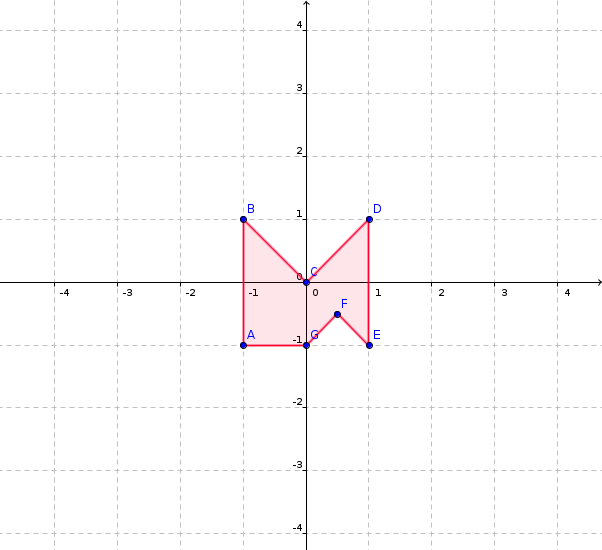
\includegraphics[width=0.35\linewidth]{images/original} \end{center}
	\begin{multicols}{2}
	\begin{enumerate} [label=(\alph*)]
		\item ~\vspace{-5mm} \\ 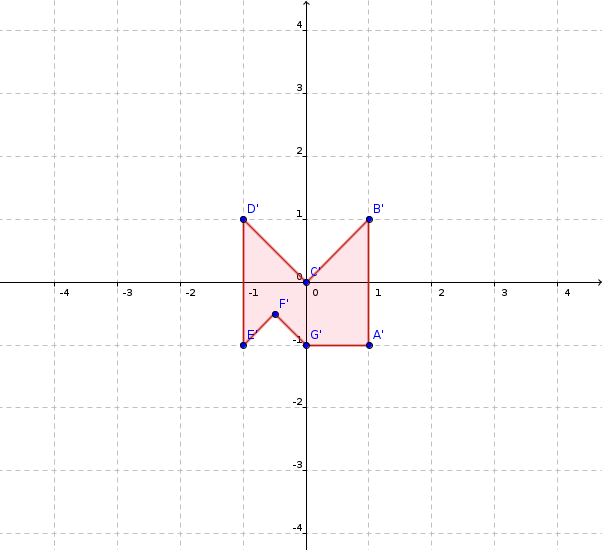
\includegraphics[width=0.7\linewidth]{images/1}
		\item ~\vspace{-5mm} \\ 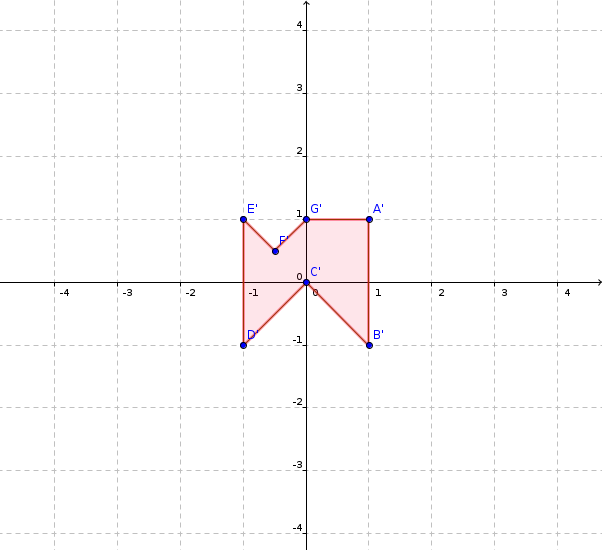
\includegraphics[width=0.7\linewidth]{images/2}
		\item ~\vspace{-5mm} \\ 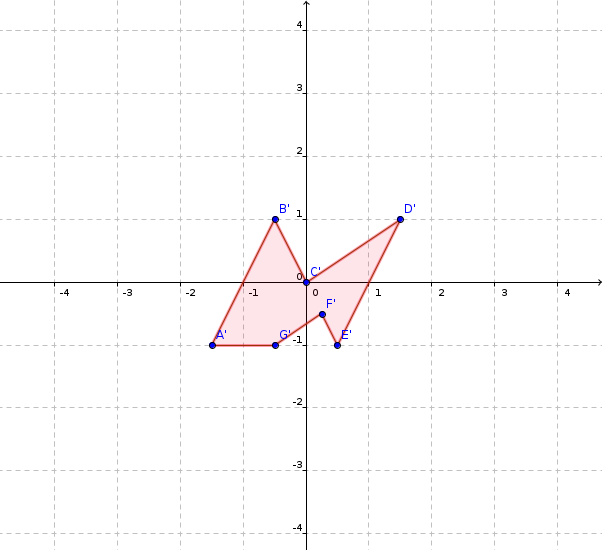
\includegraphics[width=0.7\linewidth]{images/3}
		\item ~\vspace{-5mm} \\ 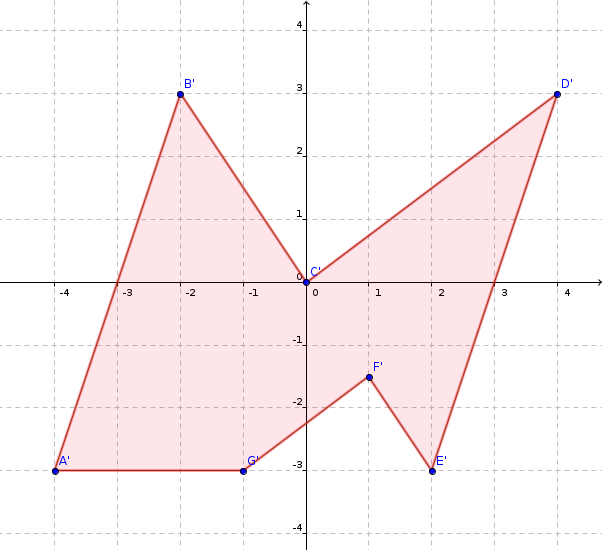
\includegraphics[width=0.7\linewidth]{images/4}
		\item ~\vspace{-5mm} \\ 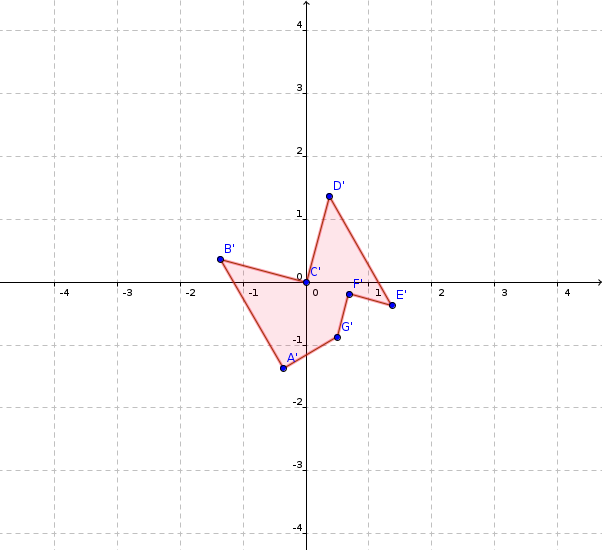
\includegraphics[width=0.7\linewidth]{images/5}
		\item ~\vspace{-5mm} \\ 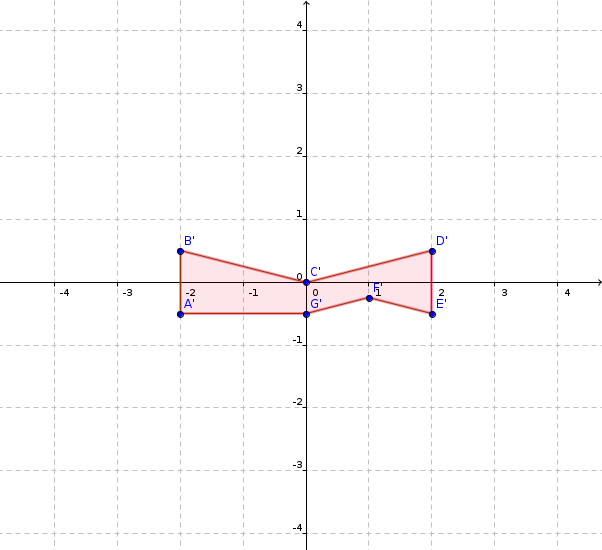
\includegraphics[width=0.7\linewidth]{images/6}
		\item ~\vspace{-5mm} \\ 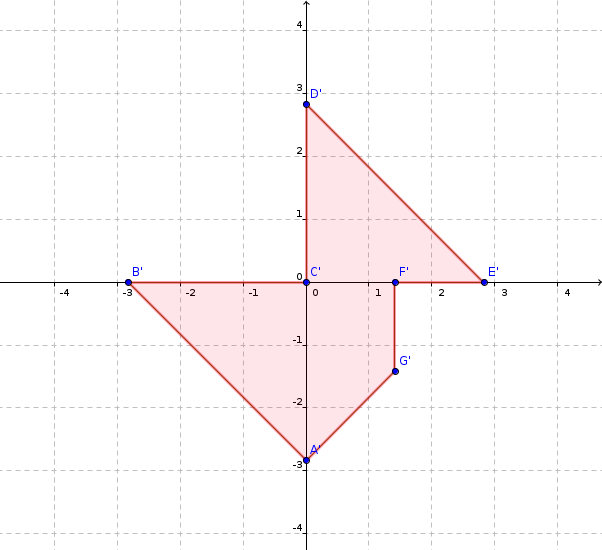
\includegraphics[width=0.7\linewidth]{images/7}
		\item ~\vspace{-5mm}\\ 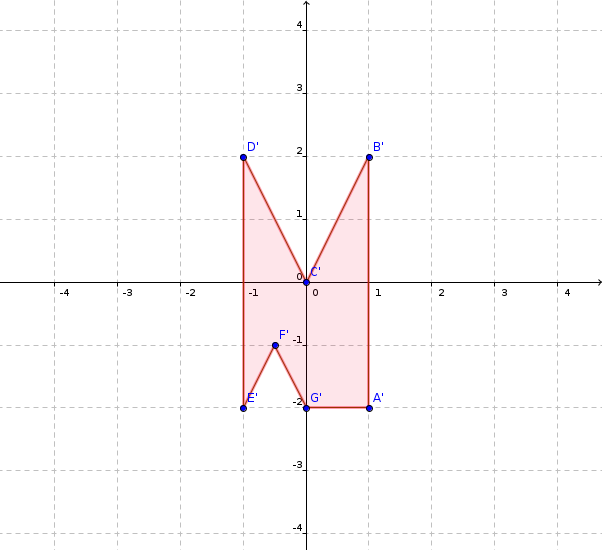
\includegraphics[width=0.7\linewidth]{images/8}
		\item ~\vspace{-5mm} \\ 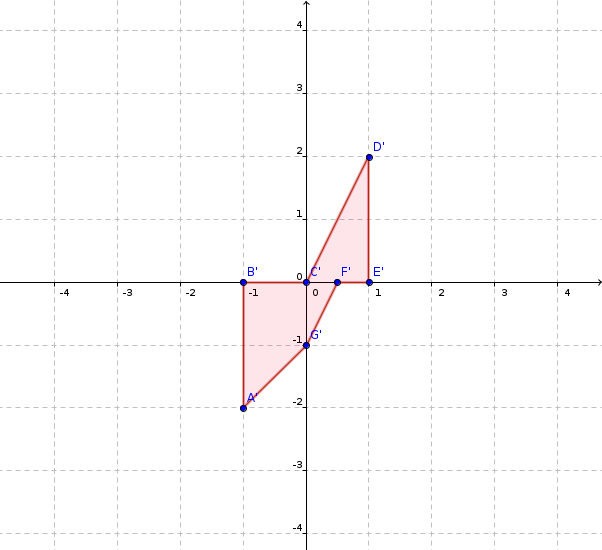
\includegraphics[width=0.7\linewidth]{images/9}
	\end{enumerate}
	\end{multicols}
	%\exercise En caso de que sea posible, resolver los siguientes sistemas de ecuaciones utilizando matrices.
	%\begin{multicols}{2}
	%\begin{enumerate} [label=(\alph*)]
	%	\item $\left\{ \begin{matrix} 3x+4y-2z=2 \\ x-z=-3 \\ 3x+5y-2z=1 \end{matrix} \right.$ 
	%	\answer ~
	%\end{enumerate}
	%\end{multicols}
\end{enumerate}
\vspace{20pt} 
 \textbf{Respuestas}\begin{enumerate}\exercise\begin{enumerate} [label=(\alph*)]		\item $A+B=\left(\begin{matrix} -1 & 2+4i & 2i\\ -1-i & 3-2i & 2+i \end{matrix}\right)$. Resolución en \href{https://youtu.be/On25s6Z1DM4}{este link}.
		\item $\frac{2}{5}B=\left(\begin{matrix} -\frac{4}{5} & \frac{8}{5}i & 0\\ \frac{2}{5}i & \frac{6}{5} & \frac{4}{5}i \end{matrix}\right)$. Resolución en \href{https://youtu.be/On25s6Z1DM4}{este link}.
		\item $2B=\left(\begin{matrix} 4 & -8i & 0\\ -2i & -6 & -4i \end{matrix}\right)$. Resolución en \href{https://youtu.be/On25s6Z1DM4}{este link}.
		\item $A^T+2B^T=\left(\begin{matrix} 3 & -1+2i\\ 2+8i & 6-2i \\ 2i & 2+4i \end{matrix}\right)$. Resolución en \href{https://youtu.be/On25s6Z1DM4}{este link}.
		\item $A^T-B^T=\left(\begin{matrix} 3 & -1-i\\ 2-4i & -3-2i \\ 2i & 2-2i \end{matrix}\right)$. Resolución en \href{https://youtu.be/On25s6Z1DM4}{este link}.
		\item $A^T-B^T=\left(\begin{matrix} 3 & -1-i\\ 2-4i & -3-2i \\ 2i & 2-2i \end{matrix}\right)$.
		\item $A5\overline{A}=\left(\begin{matrix} 5 & 10 & -10i\\ -5 & 10i & 10 \end{matrix}\right)$.
		\item $A+B^{\dagger}=\left(\begin{matrix} -1 & -1-i\\ 2+4i & 3-2i \\ 2i & 2-2i \end{matrix}\right)$.
		\item No es posible, ya que A tiene tamaño 2x3 y $B^{\dagger}$ tiene tamaño 3x2. 
\end{enumerate}\exercise\begin{enumerate} [label=(\alph*)]		\item Resolución en \href{https://youtu.be/-55zVuwssEs}{este link}.
		\item No se puede, ya que $A^T$ es 2x3 y $B^T$ es 2x2.
		\item Resolución en \href{https://youtu.be/-55zVuwssEs}{este link}.
		\item Resolución en \href{https://youtu.be/-55zVuwssEs}{este link}.
		\item $B^2=\left(\begin{matrix} 1 & -3\\ 0 & 4 \end{matrix}\right)$
		\item $B^3=\left(\begin{matrix} 1 & -7\\ 0 & 8 \end{matrix}\right)$
		\item $A.B^2=\left(\begin{matrix} 2 & -2\\ -2 & 10 \\ 1 & 9 \end{matrix}\right)$
		\item No se puede, ya que $2A$ es 3x2 y $B$ es 2x2.
		\item No se puede calcular $B.A$ ya que $B$ es 2x2 y $A$ es 3x2.
		\item $B^2 - A^T.A=\left(\begin{matrix} -8 & -6\\ -3 & -7 \end{matrix}\right)$
		\item No se puede calcular $A^2$ ya que 3x2, por lo tanto tampoco $A^3$.
		\item $E^T-2E^2=\left(\begin{matrix} 3 & 0 & -4 \\ 0 & 3 & -20 \\ -1 & -5 & 3 \end{matrix}\right)$ 
		\item $5A-E.(A^T)^T=\left(\begin{matrix} 9 & 7\\ -3 & 19 \\ 4 & 12 \end{matrix}\right)$
		\item No se puede calcular $A.D$ ya que $A$ es 3x2 y $D$ es 3x1.
		\item $C.D=\left(\begin{matrix} -2 \end{matrix}\right)$
		\item $D.C=\left(\begin{matrix} -2 & 0 & -4 \\ -1 & 0 & -2 \\ 0 & 0 & 0 \end{matrix}\right)$
		\item $E.D-D=\left(\begin{matrix} 0 \\ 0 \\ 0 \end{matrix}\right)$
		\item $C.E+C=\left(\begin{matrix} 2 & 0 & 3 \end{matrix}\right)$
\end{enumerate}\exercise\begin{enumerate} [label=(\alph*)]		\item $(x,y,z)=(3,-4,-4)$. Resolución por \href{https://youtu.be/hIkRaA2IfQ8?t=328}{Aprende Matemáticas}.
		\item $\left(\alpha,\beta,\gamma,\delta\right)=(2,-3,\frac{7}{2},-1)$. Resolución por \href{https://youtu.be/ENijHEsXKoc}{Mate Profesor Rosado}.
		\item Existen dos soluciones: $(x,y,z)=(-6,-3,3)$ y también $(x,y,z)=(-6,2,3)$. El conjunto solución es $S=\left\{(-6,-3,3),(-6,2,3)\right\}$. Resolución por \href{https://youtu.be/3WSRu7shF4s}{Matemática Serie 23}.
		\item $(a,b,c)=(6,0,3)$. Resolución por \href{https://youtu.be/L1cAscCfFmU}{Rolando Flores Aguilar}.
		\item Existen dos soluciones: $(x,y)=(3,-2)$ y también $(x,y)=(-2,3)$. El conjunto solución es $S=\left\{(-2,3),(3,-2)\right\}$. Resolución por \href{https://youtu.be/wj-r4isFDN4}{Mates con Andrés}.
\end{enumerate}\exercise\begin{enumerate} [label=(\alph*)]		\item ~
		\item ~
		\item ~
		\item ~
		\item ~
		\item ~
		\item ~
		\item ~
		\item ~
		\item ~
\end{enumerate}\exercise\begin{enumerate} [label=(\alph*)]		\item $X=B.A + 2 C.B^T.A - I$. Resolución por \href{https://youtu.be/U8HIvdPMNCk}{Matías Hugo Cerrudo}.
		\item $X=D^T - E^T$. Resolución por \href{https://youtu.be/6KheMCVO_r0}{Jordy Lanzas}.
		\item ~
		\item Resolución en \href{https://youtu.be/FJoaFy4OIRo}{este link}.
		\item Resolución en \href{https://youtu.be/5AU3jEAnowU?t=334}{este link}.
		\item ~
		\item ~.
		\item ~.
\end{enumerate}\exercise\begin{enumerate} [label=(\alph*)]		\item Resolución por \href{https://youtu.be/G-f-VBTi-4A}{Programa Matemática DuocUC}.
		\item Resolución en \href{https://youtu.be/kvQwypiR71o}{este link}.
		\item Resolución por \href{https://youtu.be/qnA7d-AoodE}{TuCiencia 2}
		\item La planta A tiene menor utilidad al generar \$7000 al mes. El modelo M1 tiene menor utilidad al generar \$3000 mensuales. La linea de producción de menor utilidad es el modelo M1 en la planta A, que genera \$1000 mensuales. Resolución por \href{https://youtu.be/aPGgIhqe96U}{TuCiencia 2}
		\item Masas: $M=\left(\begin{matrix} 27,976927 & 28,976495 & 29,973770 \end{matrix}\right)$. Abundancias: $A=\left(\begin{matrix} 92,2297 \\ 4,6832 \\ 3,0872 \end{matrix}\right)$. Mása atómica promedio: $M.\frac{1}{100}A=28.0854132826$.
\end{enumerate}\exercise\begin{enumerate} [label=(\alph*)]		\item
		\item
		\item
		\item
		\item
		\item
		\item
		\item
		\item
\end{enumerate}\end{enumerate}\end{document}